\documentclass[11pt]{beamer}
\usepackage{mathtools, enumerate, graphicx, cancel}

\usetheme[hideothersubsections]{Hannover}
\usecolortheme{dolphin}
\setbeamercovered{invisible}
\setbeamertemplate{navigation symbols}{\insertslidenavigationsymbol}
\setbeamertemplate{page number in head/foot}{}
\setbeamertemplate{blocks}[rounded][shadow=false]
% \setbeamerfont{section in sidebar}{size=\fontsize{4}{3}\selectfont}
% \setbeamerfont{subsection in sidebar}{size=\fontsize{4}{3}\selectfont}
% \setbeamerfont{subsubsection in sidebar}{size=\fontsize{4}{2}\selectfont}

\AtBeginSection[]{}
\AtBeginSection[]{
  \begin{frame}
    \vfill
    \centering
    \begin{beamercolorbox}[sep=8pt,center,shadow=true,rounded=true]{title}
    \usebeamerfont{title}\insertsectionhead\par%
    \end{beamercolorbox}
    \vfill
  \end{frame}
}

\AtBeginSubsection[]{
  \begin{frame}
    \vfill
    \centering
    \begin{beamercolorbox}[sep=8pt,center,shadow=true,rounded=true]{title}
    \usebeamerfont{title}\insertsectionhead\par%
    \usebeamerfont{subtitle}\insertsubsectionhead\par%
    \end{beamercolorbox}
    \vfill
  \end{frame}
}
\begin{document}

\title{Welcome to Quarantine Trivia!}
\date{}

\begin{frame}
\titlepage{}
\end{frame}

\begingroup{}
\begin{frame}
\vfill{}
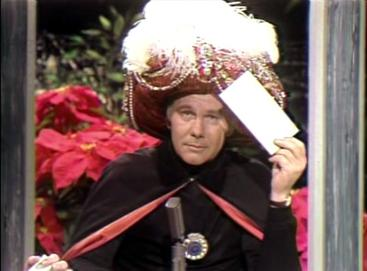
\includegraphics[width=0.7\linewidth,scale=0.7]{carson.JPG}
\centering{}
\begin{beamercolorbox}[sep=8pt,center,shadow=true,rounded=true]{title}
\usebeamerfont{title}To ensure fairness, the answers have been kept in a mayonnaise jar on Funk \& Wagnalls’ porch since noon today.
\end{beamercolorbox}
\vfill{}
\end{frame}
\endgroup{}

\begingroup{}
\begin{frame}
\vfill{}
\begin{beamercolorbox}[sep=8pt,center,shadow=true,rounded=true]{title}
\usebeamerfont{title}Good luck everyone! And have fun!
\end{beamercolorbox}
\vfill{}
\end{frame}
\endgroup{}
    

\section{Round 1}
    

\subsection*{Q1}
\begin{frame}[t]{Round 1, Question 1}
\vspace{2em}
\begin{block}{Question}
What band from Athens, Georgia featured Peter Buck, Mike Mills, Bill Berry, \& Michael Stipe\@?
\end{block}
\end{frame}
    

\subsection*{Q2}
\begin{frame}[t]{Round 1, Question 2}
\vspace{2em}
\begin{block}{Question}
What constellation, also called the ``Chained Lady'', is found in the fall in the skies of the Northern Hemisphere\@?
\end{block}
\end{frame}
    

\subsection*{Q3}
\begin{frame}[t]{Round 1, Question 3}
\vspace{2em}
\begin{block}{Question}
Which composer brought ``Cats'', ``The Phantom of the Opera'' and ``Evita'' to the musical stage\@?
\end{block}
\end{frame}
    

\subsection*{Q4}
\begin{frame}[t]{Round 1, Question 4}
\vspace{2em}
\begin{block}{Question}
What popular video sharing platform was shut down in late 2016\@?
\end{block}
\end{frame}
    

\subsection*{Q5}
\begin{frame}[t]{Round 1, Question 5}
\vspace{2em}
\begin{block}{Question}
The royal families of what two countries fought for power and control during the 100 Years War\@?
\end{block}
\end{frame}
    

\subsection*{Q6}
\begin{frame}[t]{Round 1, Question 6}
\vspace{2em}
\begin{block}{Question}
What breed of large, often brown and white dog shares its name with a Japanese prefecture\@?
\end{block}
\end{frame}
    

\subsection*{Q7}
\begin{frame}[t]{Round 1, Question 7}
\vspace{2em}
\begin{block}{Question}
Three of the top six Fortune 500 companies in the US in 2014 were all in the same business. What business were these companies in\@?
\end{block}
\end{frame}
    

\subsection*{Q8}
\begin{frame}[t]{Round 1, Question 8}
\vspace{2em}
\begin{block}{Question}
What Boris Pasternak literary classic was turned into a film with Omar Sharif in the title role\@?
\end{block}
\end{frame}
    

\subsection*{Q9}
\begin{frame}[t]{Round 1, Question 9}
\vspace{2em}
\begin{block}{Question}
From the French meaning ``on equal terms'', what two word phrase is used for a foreigner who comes to another country to take care of people's children\@?
\end{block}
\end{frame}
    

\subsection*{Q10}
\begin{frame}[t]{Round 1, Question 10}
\vspace{2em}
\begin{block}{Question}
What future English king won the Battle of Hastings in 1066 leading the Norman forces\@?
\end{block}
\end{frame}
    
\subsection{Answers}

\begin{frame}[t]{Round 1, Answer 1}
\vspace{2em}
\begin{block}{Question}
What band from Athens, Georgia featured Peter Buck, Mike Mills, Bill Berry, \& Michael Stipe\@?
\end{block}
\pause{}
\begin{block}{Answer}
R.E.M.
\end{block}
\end{frame}
    

\begin{frame}[t]{Round 1, Answer 2}
\vspace{2em}
\begin{block}{Question}
What constellation, also called the ``Chained Lady'', is found in the fall in the skies of the Northern Hemisphere\@?
\end{block}
\pause{}
\begin{block}{Answer}
Andromeda
\end{block}
\end{frame}
    

\begin{frame}[t]{Round 1, Answer 3}
\vspace{2em}
\begin{block}{Question}
Which composer brought ``Cats'', ``The Phantom of the Opera'' and ``Evita'' to the musical stage\@?
\end{block}
\pause{}
\begin{block}{Answer}
Andrew Lloyd Webber
\end{block}
\end{frame}
    

\begin{frame}[t]{Round 1, Answer 4}
\vspace{2em}
\begin{block}{Question}
What popular video sharing platform was shut down in late 2016\@?
\end{block}
\pause{}
\begin{block}{Answer}
Vine
\end{block}
\end{frame}
    

\begin{frame}[t]{Round 1, Answer 5}
\vspace{2em}
\begin{block}{Question}
The royal families of what two countries fought for power and control during the 100 Years War\@?
\end{block}
\pause{}
\begin{block}{Answer}
England and France
\end{block}
\end{frame}
    

\begin{frame}[t]{Round 1, Answer 6}
\vspace{2em}
\begin{block}{Question}
What breed of large, often brown and white dog shares its name with a Japanese prefecture\@?
\end{block}
\pause{}
\begin{block}{Answer}
Akita
\end{block}
\end{frame}
    

\begin{frame}[t]{Round 1, Answer 7}
\vspace{2em}
\begin{block}{Question}
Three of the top six Fortune 500 companies in the US in 2014 were all in the same business. What business were these companies in\@?
\end{block}
\pause{}
\begin{block}{Answer}
Oil
\end{block}
\end{frame}
    

\begin{frame}[t]{Round 1, Answer 8}
\vspace{2em}
\begin{block}{Question}
What Boris Pasternak literary classic was turned into a film with Omar Sharif in the title role\@?
\end{block}
\pause{}
\begin{block}{Answer}
Doctor Zhivago
\end{block}
\end{frame}
    

\begin{frame}[t]{Round 1, Answer 9}
\vspace{2em}
\begin{block}{Question}
From the French meaning ``on equal terms'', what two word phrase is used for a foreigner who comes to another country to take care of people's children\@?
\end{block}
\pause{}
\begin{block}{Answer}
Au pair
\end{block}
\end{frame}
    

\begin{frame}[t]{Round 1, Answer 10}
\vspace{2em}
\begin{block}{Question}
What future English king won the Battle of Hastings in 1066 leading the Norman forces\@?
\end{block}
\pause{}
\begin{block}{Answer}
William the Conqueror
\end{block}
\end{frame}
    

\section{Round 2}
    

\subsection*{Q1}
\begin{frame}[t]{Round 2, Question 1}
\vspace{2em}
\begin{block}{Question}
What country is the only country in the world named after a chemical element, specifically the Latin word for silver\@?
\end{block}
\end{frame}
    

\subsection*{Q2}
\begin{frame}[t]{Round 2, Question 2}
\vspace{2em}
\begin{block}{Question}
In what Shakespearean play do both title characters die, one by the sword and one by an asp\@?
\end{block}
\end{frame}
    

\subsection*{Q3}
\begin{frame}[t]{Round 2, Question 3}
\vspace{2em}
\begin{block}{Question}
What military campaign launched by the Viet Cong in early 1968 is named for the lunar new year\@?
\end{block}
\end{frame}
    

\subsection*{Q4}
\begin{frame}[t]{Round 2, Question 4}
\vspace{2em}
\begin{block}{Question}
What was the name of the first dog in space\@?
\end{block}
\end{frame}
    

\subsection*{Q5}
\begin{frame}[t]{Round 2, Question 5}
\vspace{2em}
\begin{block}{Question}
What District 4 victor, who won at the age of 14, is an ally of Katniss Everdeen and wields a trident\@?
\end{block}
\end{frame}
    

\subsection*{Q6}
\begin{frame}[t]{Round 2, Question 6}
\vspace{2em}
\begin{block}{Question}
What is the top-selling album of all time\@?
\end{block}
\end{frame}
    

\subsection*{Q7}
\begin{frame}[t]{Round 2, Question 7}
\vspace{2em}
\begin{block}{Question}
What is the name of the luxury car division of the Honda Motor Company\@?
\end{block}
\end{frame}
    

\subsection*{Q8}
\begin{frame}[t]{Round 2, Question 8}
\vspace{2em}
\begin{block}{Question}
All Saints' Day is celebrated on the first day of what month\@?
\end{block}
\end{frame}
    

\subsection*{Q9}
\begin{frame}[t]{Round 2, Question 9}
\vspace{2em}
\begin{block}{Question}
What is the sequel to the movie Alien\@?
\end{block}
\end{frame}
    

\subsection*{Q10}
\begin{frame}[t]{Round 2, Question 10}
\vspace{2em}
\begin{block}{Question}
What code, which means literally ``the way of the warrior'', was followed by the samurai\@?
\end{block}
\end{frame}
    
\subsection{Answers}

\begin{frame}[t]{Round 2, Answer 1}
\vspace{2em}
\begin{block}{Question}
What country is the only country in the world named after a chemical element, specifically the Latin word for silver\@?
\end{block}
\pause{}
\begin{block}{Answer}
Argentina (argentum)
\end{block}
\end{frame}
    

\begin{frame}[t]{Round 2, Answer 2}
\vspace{2em}
\begin{block}{Question}
In what Shakespearean play do both title characters die, one by the sword and one by an asp\@?
\end{block}
\pause{}
\begin{block}{Answer}
Antony and Cleopatra
\end{block}
\end{frame}
    

\begin{frame}[t]{Round 2, Answer 3}
\vspace{2em}
\begin{block}{Question}
What military campaign launched by the Viet Cong in early 1968 is named for the lunar new year\@?
\end{block}
\pause{}
\begin{block}{Answer}
Tet Offensive
\end{block}
\end{frame}
    

\begin{frame}[t]{Round 2, Answer 4}
\vspace{2em}
\begin{block}{Question}
What was the name of the first dog in space\@?
\end{block}
\pause{}
\begin{block}{Answer}
Laika
\end{block}
\end{frame}
    

\begin{frame}[t]{Round 2, Answer 5}
\vspace{2em}
\begin{block}{Question}
What District 4 victor, who won at the age of 14, is an ally of Katniss Everdeen and wields a trident\@?
\end{block}
\pause{}
\begin{block}{Answer}
Finnick
\end{block}
\end{frame}
    

\begin{frame}[t]{Round 2, Answer 6}
\vspace{2em}
\begin{block}{Question}
What is the top-selling album of all time\@?
\end{block}
\pause{}
\begin{block}{Answer}
Michael Jackson's Thriller
\end{block}
\end{frame}
    

\begin{frame}[t]{Round 2, Answer 7}
\vspace{2em}
\begin{block}{Question}
What is the name of the luxury car division of the Honda Motor Company\@?
\end{block}
\pause{}
\begin{block}{Answer}
Acura
\end{block}
\end{frame}
    

\begin{frame}[t]{Round 2, Answer 8}
\vspace{2em}
\begin{block}{Question}
All Saints' Day is celebrated on the first day of what month\@?
\end{block}
\pause{}
\begin{block}{Answer}
November. (It is also known as All Hallows' Day -- the day Halloween is the eve of.)
\end{block}
\end{frame}
    

\begin{frame}[t]{Round 2, Answer 9}
\vspace{2em}
\begin{block}{Question}
What is the sequel to the movie Alien\@?
\end{block}
\pause{}
\begin{block}{Answer}
Aliens
\end{block}
\end{frame}
    

\begin{frame}[t]{Round 2, Answer 10}
\vspace{2em}
\begin{block}{Question}
What code, which means literally ``the way of the warrior'', was followed by the samurai\@?
\end{block}
\pause{}
\begin{block}{Answer}
Bushido
\end{block}
\end{frame}
    

\section{Round 3}
    

\subsection*{Q1}
\begin{frame}[t]{Round 3, Question 1}
\vspace{2em}
\begin{block}{Question}
What is the name of the princess who Disney refers to as Sleeping Beauty or Briar Rose\@?
\end{block}
\end{frame}
    

\subsection*{Q2}
\begin{frame}[t]{Round 3, Question 2}
\vspace{2em}
\begin{block}{Question}
What American figure skater and 1988 Olympic champion is featured as a recurring character in South Park\@?
\end{block}
\end{frame}
    

\subsection*{Q3}
\begin{frame}[t]{Round 3, Question 3}
\vspace{2em}
\begin{block}{Question}
What is the largest river in the world by volume of water discharged annually\@?
\end{block}
\end{frame}
    

\subsection*{Q4}
\begin{frame}[t]{Round 3, Question 4}
\vspace{2em}
\begin{block}{Question}
In Greek mythology, Stheno, Euryale, and Medusa are what kind of monster that can turn living things to stone\@?
\end{block}
\end{frame}
    

\subsection*{Q5}
\begin{frame}[t]{Round 3, Question 5}
\vspace{2em}
\begin{block}{Question}
What highly toxic poison, used in several terror attacks, is made from castor beans\@?
\end{block}
\end{frame}
    

\subsection*{Q6}
\begin{frame}[t]{Round 3, Question 6}
\vspace{2em}
\begin{block}{Question}
Which part of a gun shares its name with Roy Rogers's horse\@?
\end{block}
\end{frame}
    

\subsection*{Q7}
\begin{frame}[t]{Round 3, Question 7}
\vspace{2em}
\begin{block}{Question}
Angry Birds is a popular game produced by Rovio Mobile. In what country is Rovio based\@?
\end{block}
\end{frame}
    

\subsection*{Q8}
\begin{frame}[t]{Round 3, Question 8}
\vspace{2em}
\begin{block}{Question}
What type of building was Don Quixote jousting with thinking they were giants\@?
\end{block}
\end{frame}
    

\subsection*{Q9}
\begin{frame}[t]{Round 3, Question 9}
\vspace{2em}
\begin{block}{Question}
What is the surname of Romeo in the Shakespearean play ``Romeo and Juliet''\@?
\end{block}
\end{frame}
    

\subsection*{Q10}
\begin{frame}[t]{Round 3, Question 10}
\vspace{2em}
\begin{block}{Question}
What English poet is most noted for ``Kubla Khan'' and ``The Rime of the Ancient Mariner''\@?
\end{block}
\end{frame}
    
\subsection{Answers}

\begin{frame}[t]{Round 3, Answer 1}
\vspace{2em}
\begin{block}{Question}
What is the name of the princess who Disney refers to as Sleeping Beauty or Briar Rose\@?
\end{block}
\pause{}
\begin{block}{Answer}
Aurora
\end{block}
\end{frame}
    

\begin{frame}[t]{Round 3, Answer 2}
\vspace{2em}
\begin{block}{Question}
What American figure skater and 1988 Olympic champion is featured as a recurring character in South Park\@?
\end{block}
\pause{}
\begin{block}{Answer}
Brian Boitano
\end{block}
\end{frame}
    

\begin{frame}[t]{Round 3, Answer 3}
\vspace{2em}
\begin{block}{Question}
What is the largest river in the world by volume of water discharged annually\@?
\end{block}
\pause{}
\begin{block}{Answer}
Amazon
\end{block}
\end{frame}
    

\begin{frame}[t]{Round 3, Answer 4}
\vspace{2em}
\begin{block}{Question}
In Greek mythology, Stheno, Euryale, and Medusa are what kind of monster that can turn living things to stone\@?
\end{block}
\pause{}
\begin{block}{Answer}
Gorgon
\end{block}
\end{frame}
    

\begin{frame}[t]{Round 3, Answer 5}
\vspace{2em}
\begin{block}{Question}
What highly toxic poison, used in several terror attacks, is made from castor beans\@?
\end{block}
\pause{}
\begin{block}{Answer}
Ricin
\end{block}
\end{frame}
    

\begin{frame}[t]{Round 3, Answer 6}
\vspace{2em}
\begin{block}{Question}
Which part of a gun shares its name with Roy Rogers's horse\@?
\end{block}
\pause{}
\begin{block}{Answer}
Trigger
\end{block}
\end{frame}
    

\begin{frame}[t]{Round 3, Answer 7}
\vspace{2em}
\begin{block}{Question}
Angry Birds is a popular game produced by Rovio Mobile. In what country is Rovio based\@?
\end{block}
\pause{}
\begin{block}{Answer}
Finland
\end{block}
\end{frame}
    

\begin{frame}[t]{Round 3, Answer 8}
\vspace{2em}
\begin{block}{Question}
What type of building was Don Quixote jousting with thinking they were giants\@?
\end{block}
\pause{}
\begin{block}{Answer}
Windmill
\end{block}
\end{frame}
    

\begin{frame}[t]{Round 3, Answer 9}
\vspace{2em}
\begin{block}{Question}
What is the surname of Romeo in the Shakespearean play ``Romeo and Juliet''\@?
\end{block}
\pause{}
\begin{block}{Answer}
Montague
\end{block}
\end{frame}
    

\begin{frame}[t]{Round 3, Answer 10}
\vspace{2em}
\begin{block}{Question}
What English poet is most noted for ``Kubla Khan'' and ``The Rime of the Ancient Mariner''\@?
\end{block}
\pause{}
\begin{block}{Answer}
Samuel Coleridge
\end{block}
\end{frame}
    

\section{Round 4}
    

\subsection*{Q1}
\begin{frame}[t]{Round 4, Question 1}
\vspace{2em}
\begin{block}{Question}
What is the name of the largest artery in the human body\@?
\end{block}
\end{frame}
    

\subsection*{Q2}
\begin{frame}[t]{Round 4, Question 2}
\vspace{2em}
\begin{block}{Question}
The United Nations controls the International Court of Justice. In what country is the ICJ headquartered\@?
\end{block}
\end{frame}
    

\subsection*{Q3}
\begin{frame}[t]{Round 4, Question 3}
\vspace{2em}
\begin{block}{Question}
What flower of the narcissus genus, which is often yellow and trumpet shaped, was honored in a Wordsworth poem\@?
\end{block}
\end{frame}
    

\subsection*{Q4}
\begin{frame}[t]{Round 4, Question 4}
\vspace{2em}
\begin{block}{Question}
What powerful opiate drug is named after the Greek god of dreams\@?
\end{block}
\end{frame}
    

\subsection*{Q5}
\begin{frame}[t]{Round 4, Question 5}
\vspace{2em}
\begin{block}{Question}
What TV clown first appeared in 1949, and has been played by many people including Willard Scott\@?
\end{block}
\end{frame}
    

\subsection*{Q6}
\begin{frame}[t]{Round 4, Question 6}
\vspace{2em}
\begin{block}{Question}
What neighborhood of northwest Washington, DC, gives its name to the State Department because it is located there\@?
\end{block}
\end{frame}
    

\subsection*{Q7}
\begin{frame}[t]{Round 4, Question 7}
\vspace{2em}
\begin{block}{Question}
What was Elvis Presley's middle name\@?
\end{block}
\end{frame}
    

\subsection*{Q8}
\begin{frame}[t]{Round 4, Question 8}
\vspace{2em}
\begin{block}{Question}
Who was the first Founding Father to sign the Declaration of Independence\@?
\end{block}
\end{frame}
    

\subsection*{Q9}
\begin{frame}[t]{Round 4, Question 9}
\vspace{2em}
\begin{block}{Question}
What type of animal is Pumbaa in ``The Lion King''\@?
\end{block}
\end{frame}
    

\subsection*{Q10}
\begin{frame}[t]{Round 4, Question 10}
\vspace{2em}
\begin{block}{Question}
What Tony-winning musical features a pseudo-historical plot involving characters named Charlemagne and his titular real-life son\@?
\end{block}
\end{frame}
    
\subsection{Answers}

\begin{frame}[t]{Round 4, Answer 1}
\vspace{2em}
\begin{block}{Question}
What is the name of the largest artery in the human body\@?
\end{block}
\pause{}
\begin{block}{Answer}
Aorta
\end{block}
\end{frame}
    

\begin{frame}[t]{Round 4, Answer 2}
\vspace{2em}
\begin{block}{Question}
The United Nations controls the International Court of Justice. In what country is the ICJ headquartered\@?
\end{block}
\pause{}
\begin{block}{Answer}
The Netherlands
\end{block}
\end{frame}
    

\begin{frame}[t]{Round 4, Answer 3}
\vspace{2em}
\begin{block}{Question}
What flower of the narcissus genus, which is often yellow and trumpet shaped, was honored in a Wordsworth poem\@?
\end{block}
\pause{}
\begin{block}{Answer}
Daffodil
\end{block}
\end{frame}
    

\begin{frame}[t]{Round 4, Answer 4}
\vspace{2em}
\begin{block}{Question}
What powerful opiate drug is named after the Greek god of dreams\@?
\end{block}
\pause{}
\begin{block}{Answer}
Morphine
\end{block}
\end{frame}
    

\begin{frame}[t]{Round 4, Answer 5}
\vspace{2em}
\begin{block}{Question}
What TV clown first appeared in 1949, and has been played by many people including Willard Scott\@?
\end{block}
\pause{}
\begin{block}{Answer}
Bozo
\end{block}
\end{frame}
    

\begin{frame}[t]{Round 4, Answer 6}
\vspace{2em}
\begin{block}{Question}
What neighborhood of northwest Washington, DC, gives its name to the State Department because it is located there\@?
\end{block}
\pause{}
\begin{block}{Answer}
Foggy Bottom
\end{block}
\end{frame}
    

\begin{frame}[t]{Round 4, Answer 7}
\vspace{2em}
\begin{block}{Question}
What was Elvis Presley's middle name\@?
\end{block}
\pause{}
\begin{block}{Answer}
Aaron
\end{block}
\end{frame}
    

\begin{frame}[t]{Round 4, Answer 8}
\vspace{2em}
\begin{block}{Question}
Who was the first Founding Father to sign the Declaration of Independence\@?
\end{block}
\pause{}
\begin{block}{Answer}
John Hancock
\end{block}
\end{frame}
    

\begin{frame}[t]{Round 4, Answer 9}
\vspace{2em}
\begin{block}{Question}
What type of animal is Pumbaa in ``The Lion King''\@?
\end{block}
\pause{}
\begin{block}{Answer}
Warthog
\end{block}
\end{frame}
    

\begin{frame}[t]{Round 4, Answer 10}
\vspace{2em}
\begin{block}{Question}
What Tony-winning musical features a pseudo-historical plot involving characters named Charlemagne and his titular real-life son\@?
\end{block}
\pause{}
\begin{block}{Answer}
Pippin
\end{block}
\end{frame}
    

\section{Round 5}
    

\subsection*{Q1}
\begin{frame}[t]{Round 5, Question 1}
\vspace{2em}
\begin{block}{Question}
``Pan's Labyrinth'' takes place during what country's fascist regime in 1944\@?
\end{block}
\end{frame}
    

\subsection*{Q2}
\begin{frame}[t]{Round 5, Question 2}
\vspace{2em}
\begin{block}{Question}
The IMF, the International Monetary Fund, is headquartered in what world capital\@?
\end{block}
\end{frame}
    

\subsection*{Q3}
\begin{frame}[t]{Round 5, Question 3}
\vspace{2em}
\begin{block}{Question}
What actor, who was in a two-decade relationship with Susan Sarandon, won an Oscar for ``Mystic River''\@?
\end{block}
\end{frame}
    

\subsection*{Q4}
\begin{frame}[t]{Round 5, Question 4}
\vspace{2em}
\begin{block}{Question}
What Greek-American director won Oscars for both ``On the Waterfront'' and ``Gentleman's Agreement''\@?
\end{block}
\end{frame}
    

\subsection*{Q5}
\begin{frame}[t]{Round 5, Question 5}
\vspace{2em}
\begin{block}{Question}
Which basketball coach is the only one to win the NCAA Championship with two different teams, Kentucky and his more recent team, Louisville\@?
\end{block}
\end{frame}
    

\subsection*{Q6}
\begin{frame}[t]{Round 5, Question 6}
\vspace{2em}
\begin{block}{Question}
What is the double-sounding capital of the territory of American Samoa\@?
\end{block}
\end{frame}
    

\subsection*{Q7}
\begin{frame}[t]{Round 5, Question 7}
\vspace{2em}
\begin{block}{Question}
What 6-letter term is given to the lighting electrician on a TV or movie set\@?
\end{block}
\end{frame}
    

\subsection*{Q8}
\begin{frame}[t]{Round 5, Question 8}
\vspace{2em}
\begin{block}{Question}
In what Leo Tolstoy classic novel does the title heroine carry on an affair with Count Vronsky\@?
\end{block}
\end{frame}
    

\subsection*{Q9}
\begin{frame}[t]{Round 5, Question 9}
\vspace{2em}
\begin{block}{Question}
Which former member of Monty Python played Q in ``Die Another Day?''
\end{block}
\end{frame}
    

\subsection*{Q10}
\begin{frame}[t]{Round 5, Question 10}
\vspace{2em}
\begin{block}{Question}
What British Prime Minister had the distinction of serving between the two terms of Winston Churchill\@?
\end{block}
\end{frame}
    
\subsection{Answers}

\begin{frame}[t]{Round 5, Answer 1}
\vspace{2em}
\begin{block}{Question}
``Pan's Labyrinth'' takes place during what country's fascist regime in 1944\@?
\end{block}
\pause{}
\begin{block}{Answer}
Spain
\end{block}
\end{frame}
    

\begin{frame}[t]{Round 5, Answer 2}
\vspace{2em}
\begin{block}{Question}
The IMF, the International Monetary Fund, is headquartered in what world capital\@?
\end{block}
\pause{}
\begin{block}{Answer}
Washington, DC
\end{block}
\end{frame}
    

\begin{frame}[t]{Round 5, Answer 3}
\vspace{2em}
\begin{block}{Question}
What actor, who was in a two-decade relationship with Susan Sarandon, won an Oscar for ``Mystic River''\@?
\end{block}
\pause{}
\begin{block}{Answer}
Tim Robbins
\end{block}
\end{frame}
    

\begin{frame}[t]{Round 5, Answer 4}
\vspace{2em}
\begin{block}{Question}
What Greek-American director won Oscars for both ``On the Waterfront'' and ``Gentleman's Agreement''\@?
\end{block}
\pause{}
\begin{block}{Answer}
Elia Kazan
\end{block}
\end{frame}
    

\begin{frame}[t]{Round 5, Answer 5}
\vspace{2em}
\begin{block}{Question}
Which basketball coach is the only one to win the NCAA Championship with two different teams, Kentucky and his more recent team, Louisville\@?
\end{block}
\pause{}
\begin{block}{Answer}
Rick Pitino
\end{block}
\end{frame}
    

\begin{frame}[t]{Round 5, Answer 6}
\vspace{2em}
\begin{block}{Question}
What is the double-sounding capital of the territory of American Samoa\@?
\end{block}
\pause{}
\begin{block}{Answer}
Pago Pago
\end{block}
\end{frame}
    

\begin{frame}[t]{Round 5, Answer 7}
\vspace{2em}
\begin{block}{Question}
What 6-letter term is given to the lighting electrician on a TV or movie set\@?
\end{block}
\pause{}
\begin{block}{Answer}
Gaffer
\end{block}
\end{frame}
    

\begin{frame}[t]{Round 5, Answer 8}
\vspace{2em}
\begin{block}{Question}
In what Leo Tolstoy classic novel does the title heroine carry on an affair with Count Vronsky\@?
\end{block}
\pause{}
\begin{block}{Answer}
Anna Karenina
\end{block}
\end{frame}
    

\begin{frame}[t]{Round 5, Answer 9}
\vspace{2em}
\begin{block}{Question}
Which former member of Monty Python played Q in ``Die Another Day?''
\end{block}
\pause{}
\begin{block}{Answer}
John Cleese
\end{block}
\end{frame}
    

\begin{frame}[t]{Round 5, Answer 10}
\vspace{2em}
\begin{block}{Question}
What British Prime Minister had the distinction of serving between the two terms of Winston Churchill\@?
\end{block}
\pause{}
\begin{block}{Answer}
Clement Attlee
\end{block}
\end{frame}
    

\section{Round 6}
    

\subsection*{Q1}
\begin{frame}[t]{Round 6, Question 1}
\vspace{2em}
\begin{block}{Question}
What Alaskan city is the final destination of the Iditarod Trail Sled Dog Race\@?
\end{block}
\end{frame}
    

\subsection*{Q2}
\begin{frame}[t]{Round 6, Question 2}
\vspace{2em}
\begin{block}{Question}
Pablo Neruda, the Nobel Prize-winning poet and politician, hailed from what South American country\@?
\end{block}
\end{frame}
    

\subsection*{Q3}
\begin{frame}[t]{Round 6, Question 3}
\vspace{2em}
\begin{block}{Question}
What did King Pelias send Jason and the Argonauts off on a quest to find\@?
\end{block}
\end{frame}
    

\subsection*{Q4}
\begin{frame}[t]{Round 6, Question 4}
\vspace{2em}
\begin{block}{Question}
What former Texas Ranger/Houston Astro pitcher holds the MLB record for most strikeouts at 5,714\@?
\end{block}
\end{frame}
    

\subsection*{Q5}
\begin{frame}[t]{Round 6, Question 5}
\vspace{2em}
\begin{block}{Question}
What is the term for an ancient Mesopotamian stepped pyramid\@?
\end{block}
\end{frame}
    

\subsection*{Q6}
\begin{frame}[t]{Round 6, Question 6}
\vspace{2em}
\begin{block}{Question}
Which of Beethoven's symphonies is called the Choral, because it features the words of Schiller's ``Ode to Joy?''
\end{block}
\end{frame}
    

\subsection*{Q7}
\begin{frame}[t]{Round 6, Question 7}
\vspace{2em}
\begin{block}{Question}
Which NASA program of unmanned probes was the first to visit the outer planets and the first to go beyond Pluto\@?
\end{block}
\end{frame}
    

\subsection*{Q8}
\begin{frame}[t]{Round 6, Question 8}
\vspace{2em}
\begin{block}{Question}
What women's tennis star, who was stabbed in 1993, was known for her on-court grunting\@?
\end{block}
\end{frame}
    

\subsection*{Q9}
\begin{frame}[t]{Round 6, Question 9}
\vspace{2em}
\begin{block}{Question}
Which Disney film features the voice of Dwayne Johnson as Maui\@?
\end{block}
\end{frame}
    

\subsection*{Q10}
\begin{frame}[t]{Round 6, Question 10}
\vspace{2em}
\begin{block}{Question}
In the X-Men movies, Patrick Stewart played this character, but his younger version was played by James McAvoy in ``X-Men: First Class.'' Name this character.
\end{block}
\end{frame}
    
\subsection{Answers}

\begin{frame}[t]{Round 6, Answer 1}
\vspace{2em}
\begin{block}{Question}
What Alaskan city is the final destination of the Iditarod Trail Sled Dog Race\@?
\end{block}
\pause{}
\begin{block}{Answer}
Nome
\end{block}
\end{frame}
    

\begin{frame}[t]{Round 6, Answer 2}
\vspace{2em}
\begin{block}{Question}
Pablo Neruda, the Nobel Prize-winning poet and politician, hailed from what South American country\@?
\end{block}
\pause{}
\begin{block}{Answer}
Chile
\end{block}
\end{frame}
    

\begin{frame}[t]{Round 6, Answer 3}
\vspace{2em}
\begin{block}{Question}
What did King Pelias send Jason and the Argonauts off on a quest to find\@?
\end{block}
\pause{}
\begin{block}{Answer}
The Golden Fleece
\end{block}
\end{frame}
    

\begin{frame}[t]{Round 6, Answer 4}
\vspace{2em}
\begin{block}{Question}
What former Texas Ranger/Houston Astro pitcher holds the MLB record for most strikeouts at 5,714\@?
\end{block}
\pause{}
\begin{block}{Answer}
Nolan Ryan
\end{block}
\end{frame}
    

\begin{frame}[t]{Round 6, Answer 5}
\vspace{2em}
\begin{block}{Question}
What is the term for an ancient Mesopotamian stepped pyramid\@?
\end{block}
\pause{}
\begin{block}{Answer}
Ziggurat
\end{block}
\end{frame}
    

\begin{frame}[t]{Round 6, Answer 6}
\vspace{2em}
\begin{block}{Question}
Which of Beethoven's symphonies is called the Choral, because it features the words of Schiller's ``Ode to Joy?''
\end{block}
\pause{}
\begin{block}{Answer}
His 9th symphony
\end{block}
\end{frame}
    

\begin{frame}[t]{Round 6, Answer 7}
\vspace{2em}
\begin{block}{Question}
Which NASA program of unmanned probes was the first to visit the outer planets and the first to go beyond Pluto\@?
\end{block}
\pause{}
\begin{block}{Answer}
Pioneer
\end{block}
\end{frame}
    

\begin{frame}[t]{Round 6, Answer 8}
\vspace{2em}
\begin{block}{Question}
What women's tennis star, who was stabbed in 1993, was known for her on-court grunting\@?
\end{block}
\pause{}
\begin{block}{Answer}
Monica Seles
\end{block}
\end{frame}
    

\begin{frame}[t]{Round 6, Answer 9}
\vspace{2em}
\begin{block}{Question}
Which Disney film features the voice of Dwayne Johnson as Maui\@?
\end{block}
\pause{}
\begin{block}{Answer}
Moana
\end{block}
\end{frame}
    

\begin{frame}[t]{Round 6, Answer 10}
\vspace{2em}
\begin{block}{Question}
In the X-Men movies, Patrick Stewart played this character, but his younger version was played by James McAvoy in ``X-Men: First Class.'' Name this character.
\end{block}
\pause{}
\begin{block}{Answer}
Professor Charles Xavier (Professor X.)
\end{block}
\end{frame}
    

\section{Round 7}
    

\subsection*{Q1}
\begin{frame}[t]{Round 7, Question 1}
\vspace{2em}
\begin{block}{Question}
Charleston is the capital city of which US state\@?
\end{block}
\end{frame}
    

\subsection*{Q2}
\begin{frame}[t]{Round 7, Question 2}
\vspace{2em}
\begin{block}{Question}
What amusement park staple premiered at the 1893 Columbian Exposition in Chicago and is named after its designer\@?
\end{block}
\end{frame}
    

\subsection*{Q3}
\begin{frame}[t]{Round 7, Question 3}
\vspace{2em}
\begin{block}{Question}
What was the currency of Austria that was replaced by the euro in 1999\@?
\end{block}
\end{frame}
    

\subsection*{Q4}
\begin{frame}[t]{Round 7, Question 4}
\vspace{2em}
\begin{block}{Question}
What actor who starred in ``The Hurt Locker'' plays Hawkeye in ``The Avengers?''
\end{block}
\end{frame}
    

\subsection*{Q5}
\begin{frame}[t]{Round 7, Question 5}
\vspace{2em}
\begin{block}{Question}
What Australian children's music group foursome has been a sensation since 1991 with songs like ``Do The Monkey''\@?
\end{block}
\end{frame}
    

\subsection*{Q6}
\begin{frame}[t]{Round 7, Question 6}
\vspace{2em}
\begin{block}{Question}
What fourteenth century Italian author named Giovanni is best known for his ``Decameron''\@?
\end{block}
\end{frame}
    

\subsection*{Q7}
\begin{frame}[t]{Round 7, Question 7}
\vspace{2em}
\begin{block}{Question}
What name is shared by a famed Greco-Egyptian astronomer and mathematician and an Egyptian royal family that included Cleopatra\@?
\end{block}
\end{frame}
    

\subsection*{Q8}
\begin{frame}[t]{Round 7, Question 8}
\vspace{2em}
\begin{block}{Question}
What Shakespearean character appears in 3 plays, Henry IV Parts 1 and 2 and The Merry Wives of Windsor\@?
\end{block}
\end{frame}
    

\subsection*{Q9}
\begin{frame}[t]{Round 7, Question 9}
\vspace{2em}
\begin{block}{Question}
In what country is La Liga the top level football league\@?
\end{block}
\end{frame}
    

\subsection*{Q10}
\begin{frame}[t]{Round 7, Question 10}
\vspace{2em}
\begin{block}{Question}
What man was the first leader of the USSR after the Russian Revolution\@?
\end{block}
\end{frame}
    
\subsection{Answers}

\begin{frame}[t]{Round 7, Answer 1}
\vspace{2em}
\begin{block}{Question}
Charleston is the capital city of which US state\@?
\end{block}
\pause{}
\begin{block}{Answer}
West Virginia
\end{block}
\end{frame}
    

\begin{frame}[t]{Round 7, Answer 2}
\vspace{2em}
\begin{block}{Question}
What amusement park staple premiered at the 1893 Columbian Exposition in Chicago and is named after its designer\@?
\end{block}
\pause{}
\begin{block}{Answer}
Ferris wheel
\end{block}
\end{frame}
    

\begin{frame}[t]{Round 7, Answer 3}
\vspace{2em}
\begin{block}{Question}
What was the currency of Austria that was replaced by the euro in 1999\@?
\end{block}
\pause{}
\begin{block}{Answer}
Schilling
\end{block}
\end{frame}
    

\begin{frame}[t]{Round 7, Answer 4}
\vspace{2em}
\begin{block}{Question}
What actor who starred in ``The Hurt Locker'' plays Hawkeye in ``The Avengers?''
\end{block}
\pause{}
\begin{block}{Answer}
Jeremy Renner
\end{block}
\end{frame}
    

\begin{frame}[t]{Round 7, Answer 5}
\vspace{2em}
\begin{block}{Question}
What Australian children's music group foursome has been a sensation since 1991 with songs like ``Do The Monkey''\@?
\end{block}
\pause{}
\begin{block}{Answer}
The Wiggles
\end{block}
\end{frame}
    

\begin{frame}[t]{Round 7, Answer 6}
\vspace{2em}
\begin{block}{Question}
What fourteenth century Italian author named Giovanni is best known for his ``Decameron''\@?
\end{block}
\pause{}
\begin{block}{Answer}
Boccaccio
\end{block}
\end{frame}
    

\begin{frame}[t]{Round 7, Answer 7}
\vspace{2em}
\begin{block}{Question}
What name is shared by a famed Greco-Egyptian astronomer and mathematician and an Egyptian royal family that included Cleopatra\@?
\end{block}
\pause{}
\begin{block}{Answer}
Ptolemy
\end{block}
\end{frame}
    

\begin{frame}[t]{Round 7, Answer 8}
\vspace{2em}
\begin{block}{Question}
What Shakespearean character appears in 3 plays, Henry IV Parts 1 and 2 and The Merry Wives of Windsor\@?
\end{block}
\pause{}
\begin{block}{Answer}
Sir John Falstaff
\end{block}
\end{frame}
    

\begin{frame}[t]{Round 7, Answer 9}
\vspace{2em}
\begin{block}{Question}
In what country is La Liga the top level football league\@?
\end{block}
\pause{}
\begin{block}{Answer}
Spain
\end{block}
\end{frame}
    

\begin{frame}[t]{Round 7, Answer 10}
\vspace{2em}
\begin{block}{Question}
What man was the first leader of the USSR after the Russian Revolution\@?
\end{block}
\pause{}
\begin{block}{Answer}
Vladimir Lenin
\end{block}
\end{frame}
    

\section{Round 8}
    

\subsection*{Q1}
\begin{frame}[t]{Round 8, Question 1}
\vspace{2em}
\begin{block}{Question}
What Latin term meaning ``behold the man'' does Pontius Pilate use when presenting Jesus\@?
\end{block}
\end{frame}
    

\subsection*{Q2}
\begin{frame}[t]{Round 8, Question 2}
\vspace{2em}
\begin{block}{Question}
What kind of animal is Rikki-Tikki-Tavi in the Rudyard Kipling story\@?
\end{block}
\end{frame}
    

\subsection*{Q3}
\begin{frame}[t]{Round 8, Question 3}
\vspace{2em}
\begin{block}{Question}
What Spanish Baroque painter of the 17th century painted for the Spanish court and is most known for his ``Las Meninas''\@?
\end{block}
\end{frame}
    

\subsection*{Q4}
\begin{frame}[t]{Round 8, Question 4}
\vspace{2em}
\begin{block}{Question}
What luxury retailer, headquartered in Seattle, has 323 stores in North America, more than its competitors like Bloomingdales or Saks\@?
\end{block}
\end{frame}
    

\subsection*{Q5}
\begin{frame}[t]{Round 8, Question 5}
\vspace{2em}
\begin{block}{Question}
What quantity, measured in Newtons, is found in physics by multiplying mass times acceleration\@?
\end{block}
\end{frame}
    

\subsection*{Q6}
\begin{frame}[t]{Round 8, Question 6}
\vspace{2em}
\begin{block}{Question}
The musician born Paul Hewson is more commonly known by what stage name\@?
\end{block}
\end{frame}
    

\subsection*{Q7}
\begin{frame}[t]{Round 8, Question 7}
\vspace{2em}
\begin{block}{Question}
Name any country that is on the island of Borneo.
\end{block}
\end{frame}
    

\subsection*{Q8}
\begin{frame}[t]{Round 8, Question 8}
\vspace{2em}
\begin{block}{Question}
What variety of grape, usually used for making red wine, is named after the 5th largest city in Iran\@?
\end{block}
\end{frame}
    

\subsection*{Q9}
\begin{frame}[t]{Round 8, Question 9}
\vspace{2em}
\begin{block}{Question}
What famous one-movement musical piece by Ravel shares its name with a genre of slow tempo Latin music\@?
\end{block}
\end{frame}
    

\subsection*{Q10}
\begin{frame}[t]{Round 8, Question 10}
\vspace{2em}
\begin{block}{Question}
What 11-letter term is used to describe the labor class, usually the lowest class in the society which has only its labor to offer to an industrialized society\@?
\end{block}
\end{frame}
    
\subsection{Answers}

\begin{frame}[t]{Round 8, Answer 1}
\vspace{2em}
\begin{block}{Question}
What Latin term meaning ``behold the man'' does Pontius Pilate use when presenting Jesus\@?
\end{block}
\pause{}
\begin{block}{Answer}
Ecce homo
\end{block}
\end{frame}
    

\begin{frame}[t]{Round 8, Answer 2}
\vspace{2em}
\begin{block}{Question}
What kind of animal is Rikki-Tikki-Tavi in the Rudyard Kipling story\@?
\end{block}
\pause{}
\begin{block}{Answer}
Mongoose
\end{block}
\end{frame}
    

\begin{frame}[t]{Round 8, Answer 3}
\vspace{2em}
\begin{block}{Question}
What Spanish Baroque painter of the 17th century painted for the Spanish court and is most known for his ``Las Meninas''\@?
\end{block}
\pause{}
\begin{block}{Answer}
Diego Velázquez
\end{block}
\end{frame}
    

\begin{frame}[t]{Round 8, Answer 4}
\vspace{2em}
\begin{block}{Question}
What luxury retailer, headquartered in Seattle, has 323 stores in North America, more than its competitors like Bloomingdales or Saks\@?
\end{block}
\pause{}
\begin{block}{Answer}
Nordstrom
\end{block}
\end{frame}
    

\begin{frame}[t]{Round 8, Answer 5}
\vspace{2em}
\begin{block}{Question}
What quantity, measured in Newtons, is found in physics by multiplying mass times acceleration\@?
\end{block}
\pause{}
\begin{block}{Answer}
Force
\end{block}
\end{frame}
    

\begin{frame}[t]{Round 8, Answer 6}
\vspace{2em}
\begin{block}{Question}
The musician born Paul Hewson is more commonly known by what stage name\@?
\end{block}
\pause{}
\begin{block}{Answer}
Bono
\end{block}
\end{frame}
    

\begin{frame}[t]{Round 8, Answer 7}
\vspace{2em}
\begin{block}{Question}
Name any country that is on the island of Borneo.
\end{block}
\pause{}
\begin{block}{Answer}
Indonesia, Malaysia, Brunei
\end{block}
\end{frame}
    

\begin{frame}[t]{Round 8, Answer 8}
\vspace{2em}
\begin{block}{Question}
What variety of grape, usually used for making red wine, is named after the 5th largest city in Iran\@?
\end{block}
\pause{}
\begin{block}{Answer}
Shiraz
\end{block}
\end{frame}
    

\begin{frame}[t]{Round 8, Answer 9}
\vspace{2em}
\begin{block}{Question}
What famous one-movement musical piece by Ravel shares its name with a genre of slow tempo Latin music\@?
\end{block}
\pause{}
\begin{block}{Answer}
Boléro
\end{block}
\end{frame}
    

\begin{frame}[t]{Round 8, Answer 10}
\vspace{2em}
\begin{block}{Question}
What 11-letter term is used to describe the labor class, usually the lowest class in the society which has only its labor to offer to an industrialized society\@?
\end{block}
\pause{}
\begin{block}{Answer}
Proletariat
\end{block}
\end{frame}
    

\section{Round 9}
    

\subsection*{Q1}
\begin{frame}[t]{Round 9, Question 1}
\vspace{2em}
\begin{block}{Question}
What is the only James Bond film to have large portions of it that take place in space\@?
\end{block}
\end{frame}
    

\subsection*{Q2}
\begin{frame}[t]{Round 9, Question 2}
\vspace{2em}
\begin{block}{Question}
The soccer player born Edson Arantes do Nascimento is better known by what name\@?
\end{block}
\end{frame}
    

\subsection*{Q3}
\begin{frame}[t]{Round 9, Question 3}
\vspace{2em}
\begin{block}{Question}
A penny or cent in the US looks coppery, but it is only 2\% copper on the outside. What metal makes up 98\% of a penny\@?
\end{block}
\end{frame}
    

\subsection*{Q4}
\begin{frame}[t]{Round 9, Question 4}
\vspace{2em}
\begin{block}{Question}
What document was signed by King John in Runnymede in 1215\@?
\end{block}
\end{frame}
    

\subsection*{Q5}
\begin{frame}[t]{Round 9, Question 5}
\vspace{2em}
\begin{block}{Question}
Which famous Dutch painter's ``Irises'' and ``Portrait of Dr.\ Gachet'' each have held the record for the most money ever paid for a single painting\@?
\end{block}
\end{frame}
    

\subsection*{Q6}
\begin{frame}[t]{Round 9, Question 6}
\vspace{2em}
\begin{block}{Question}
Which country governs Fraser Island\@?
\end{block}
\end{frame}
    

\subsection*{Q7}
\begin{frame}[t]{Round 9, Question 7}
\vspace{2em}
\begin{block}{Question}
The first Nobel Prize in Physics went to Wilhelm Röntgen for his discovery of what part of the electromagnetic spectrum\@?
\end{block}
\end{frame}
    

\subsection*{Q8}
\begin{frame}[t]{Round 9, Question 8}
\vspace{2em}
\begin{block}{Question}
In what type of internal combustion engine, named for German engineer Rudolf, does the fuel get pressurized to combust and move the piston\@?
\end{block}
\end{frame}
    

\subsection*{Q9}
\begin{frame}[t]{Round 9, Question 9}
\vspace{2em}
\begin{block}{Question}
What 1999 Julia Roberts/Hugh Grant rom com is named after an area of west London\@?
\end{block}
\end{frame}
    

\subsection*{Q10}
\begin{frame}[t]{Round 9, Question 10}
\vspace{2em}
\begin{block}{Question}
There are three types of rock. Igneous, sedimentary, and this type, named because it comes from changing one of the other two types.
\end{block}
\end{frame}
    
\subsection{Answers}

\begin{frame}[t]{Round 9, Answer 1}
\vspace{2em}
\begin{block}{Question}
What is the only James Bond film to have large portions of it that take place in space\@?
\end{block}
\pause{}
\begin{block}{Answer}
Moonraker
\end{block}
\end{frame}
    

\begin{frame}[t]{Round 9, Answer 2}
\vspace{2em}
\begin{block}{Question}
The soccer player born Edson Arantes do Nascimento is better known by what name\@?
\end{block}
\pause{}
\begin{block}{Answer}
Pelé
\end{block}
\end{frame}
    

\begin{frame}[t]{Round 9, Answer 3}
\vspace{2em}
\begin{block}{Question}
A penny or cent in the US looks coppery, but it is only 2\% copper on the outside. What metal makes up 98\% of a penny\@?
\end{block}
\pause{}
\begin{block}{Answer}
Zinc
\end{block}
\end{frame}
    

\begin{frame}[t]{Round 9, Answer 4}
\vspace{2em}
\begin{block}{Question}
What document was signed by King John in Runnymede in 1215\@?
\end{block}
\pause{}
\begin{block}{Answer}
The Magna Carta
\end{block}
\end{frame}
    

\begin{frame}[t]{Round 9, Answer 5}
\vspace{2em}
\begin{block}{Question}
Which famous Dutch painter's ``Irises'' and ``Portrait of Dr.\ Gachet'' each have held the record for the most money ever paid for a single painting\@?
\end{block}
\pause{}
\begin{block}{Answer}
Vincent Van Gogh
\end{block}
\end{frame}
    

\begin{frame}[t]{Round 9, Answer 6}
\vspace{2em}
\begin{block}{Question}
Which country governs Fraser Island\@?
\end{block}
\pause{}
\begin{block}{Answer}
Australia
\end{block}
\end{frame}
    

\begin{frame}[t]{Round 9, Answer 7}
\vspace{2em}
\begin{block}{Question}
The first Nobel Prize in Physics went to Wilhelm Röntgen for his discovery of what part of the electromagnetic spectrum\@?
\end{block}
\pause{}
\begin{block}{Answer}
X-ray
\end{block}
\end{frame}
    

\begin{frame}[t]{Round 9, Answer 8}
\vspace{2em}
\begin{block}{Question}
In what type of internal combustion engine, named for German engineer Rudolf, does the fuel get pressurized to combust and move the piston\@?
\end{block}
\pause{}
\begin{block}{Answer}
Diesel
\end{block}
\end{frame}
    

\begin{frame}[t]{Round 9, Answer 9}
\vspace{2em}
\begin{block}{Question}
What 1999 Julia Roberts/Hugh Grant rom com is named after an area of west London\@?
\end{block}
\pause{}
\begin{block}{Answer}
Notting Hill
\end{block}
\end{frame}
    

\begin{frame}[t]{Round 9, Answer 10}
\vspace{2em}
\begin{block}{Question}
There are three types of rock. Igneous, sedimentary, and this type, named because it comes from changing one of the other two types.
\end{block}
\pause{}
\begin{block}{Answer}
Metamorphic
\end{block}
\end{frame}
    

\section{Round 10}
    

\subsection*{Q1}
\begin{frame}[t]{Round 10, Question 1}
\vspace{2em}
\begin{block}{Question}
What creature from Hebrew folklore is a protective automated figure of clay and shares its name with a Gen 1 Pokémon\@?
\end{block}
\end{frame}
    

\subsection*{Q2}
\begin{frame}[t]{Round 10, Question 2}
\vspace{2em}
\begin{block}{Question}
Togo, Cameroon, and Nauru are all now independent countries. At one point, they were all colonies of what country\@?
\end{block}
\end{frame}
    

\subsection*{Q3}
\begin{frame}[t]{Round 10, Question 3}
\vspace{2em}
\begin{block}{Question}
In France, Louis XIV or Louis the Great was also known by what bright nickname\@?
\end{block}
\end{frame}
    

\subsection*{Q4}
\begin{frame}[t]{Round 10, Question 4}
\vspace{2em}
\begin{block}{Question}
What was the name of the Flintstone family pet, a purple snorkasaurus\@?
\end{block}
\end{frame}
    

\subsection*{Q5}
\begin{frame}[t]{Round 10, Question 5}
\vspace{2em}
\begin{block}{Question}
What famous child psychologist and pediatrician shares a last name with the Vulcan first officer on the USS Enterprise? (First and last name)
\end{block}
\end{frame}
    

\subsection*{Q6}
\begin{frame}[t]{Round 10, Question 6}
\vspace{2em}
\begin{block}{Question}
What Division I Philadelphia college has the Dragons for its athletic team nickname\@?
\end{block}
\end{frame}
    

\subsection*{Q7}
\begin{frame}[t]{Round 10, Question 7}
\vspace{2em}
\begin{block}{Question}
Name any of the five new sports to be added to the (now postponed) 2020 Olympics.
\end{block}
\end{frame}
    

\subsection*{Q8}
\begin{frame}[t]{Round 10, Question 8}
\vspace{2em}
\begin{block}{Question}
Which comic book villain first appeared in 1956 and was essentially a mirror image of Superman\@?
\end{block}
\end{frame}
    

\subsection*{Q9}
\begin{frame}[t]{Round 10, Question 9}
\vspace{2em}
\begin{block}{Question}
A fletcher makes arrows and a cooper makes barrels. What does a wainwright make\@?
\end{block}
\end{frame}
    

\subsection*{Q10}
\begin{frame}[t]{Round 10, Question 10}
\vspace{2em}
\begin{block}{Question}
What reddish-brown gem is the birthstone for November\@?
\end{block}
\end{frame}
    
\subsection{Answers}

\begin{frame}[t]{Round 10, Answer 1}
\vspace{2em}
\begin{block}{Question}
What creature from Hebrew folklore is a protective automated figure of clay and shares its name with a Gen 1 Pokémon\@?
\end{block}
\pause{}
\begin{block}{Answer}
Golem
\end{block}
\end{frame}
    

\begin{frame}[t]{Round 10, Answer 2}
\vspace{2em}
\begin{block}{Question}
Togo, Cameroon, and Nauru are all now independent countries. At one point, they were all colonies of what country\@?
\end{block}
\pause{}
\begin{block}{Answer}
Germany
\end{block}
\end{frame}
    

\begin{frame}[t]{Round 10, Answer 3}
\vspace{2em}
\begin{block}{Question}
In France, Louis XIV or Louis the Great was also known by what bright nickname\@?
\end{block}
\pause{}
\begin{block}{Answer}
The Sun King
\end{block}
\end{frame}
    

\begin{frame}[t]{Round 10, Answer 4}
\vspace{2em}
\begin{block}{Question}
What was the name of the Flintstone family pet, a purple snorkasaurus\@?
\end{block}
\pause{}
\begin{block}{Answer}
Dino
\end{block}
\end{frame}
    

\begin{frame}[t]{Round 10, Answer 5}
\vspace{2em}
\begin{block}{Question}
What famous child psychologist and pediatrician shares a last name with the Vulcan first officer on the USS Enterprise? (First and last name)
\end{block}
\pause{}
\begin{block}{Answer}
Benjamin Spock
\end{block}
\end{frame}
    

\begin{frame}[t]{Round 10, Answer 6}
\vspace{2em}
\begin{block}{Question}
What Division I Philadelphia college has the Dragons for its athletic team nickname\@?
\end{block}
\pause{}
\begin{block}{Answer}
Drexel
\end{block}
\end{frame}
    

\begin{frame}[t]{Round 10, Answer 7}
\vspace{2em}
\begin{block}{Question}
Name any of the five new sports to be added to the (now postponed) 2020 Olympics.
\end{block}
\pause{}
\begin{block}{Answer}
Surfing, baseball, karate, skateboarding, sport climbing
\end{block}
\end{frame}
    

\begin{frame}[t]{Round 10, Answer 8}
\vspace{2em}
\begin{block}{Question}
Which comic book villain first appeared in 1956 and was essentially a mirror image of Superman\@?
\end{block}
\pause{}
\begin{block}{Answer}
Bizarro
\end{block}
\end{frame}
    

\begin{frame}[t]{Round 10, Answer 9}
\vspace{2em}
\begin{block}{Question}
A fletcher makes arrows and a cooper makes barrels. What does a wainwright make\@?
\end{block}
\pause{}
\begin{block}{Answer}
Wagons
\end{block}
\end{frame}
    

\begin{frame}[t]{Round 10, Answer 10}
\vspace{2em}
\begin{block}{Question}
What reddish-brown gem is the birthstone for November\@?
\end{block}
\pause{}
\begin{block}{Answer}
Topaz
\end{block}
\end{frame}
    

\section{Bonus Round}
    

\subsection*{Q1}
\begin{frame}[t]{Bonus Round, Question 1}
\vspace{2em}
\begin{block}{Question}
Where were the Declaration of Independence, the Constitution, and the Bill of Rights stored during World War II\@?
\end{block}
\end{frame}
    

\subsection*{Q2}
\begin{frame}[t]{Bonus Round, Question 2}
\vspace{2em}
\begin{block}{Question}
Which country consumes the most chocolate per capita\@?
\end{block}
\end{frame}
    

\subsection*{Q3}
\begin{frame}[t]{Bonus Round, Question 3}
\vspace{2em}
\begin{block}{Question}
Which two U.S. states don't observe Daylight Saving Time\@?
\end{block}
\end{frame}
    

\subsection*{Q4}
\begin{frame}[t]{Bonus Round, Question 4}
\vspace{2em}
\begin{block}{Question}
Which country has the oldest continuously used national flag\@?
\end{block}
\end{frame}
    

\subsection*{Q5}
\begin{frame}[t]{Bonus Round, Question 5}
\vspace{2em}
\begin{block}{Question}
What was the first animated film to be nominated for Best Picture at the Academy Awards\@?
\end{block}
\end{frame}
    

\subsection*{Q6}
\begin{frame}[t]{Bonus Round, Question 6}
\vspace{2em}
\begin{block}{Question}
By area, what is the largest county in the United States\@?
\end{block}
\end{frame}
    

\subsection*{Q7}
\begin{frame}[t]{Bonus Round, Question 7}
\vspace{2em}
\begin{block}{Question}
Which country is nicknamed the ``Land of a Thousand Smiles?''
\end{block}
\end{frame}
    

\subsection*{Q8}
\begin{frame}[t]{Bonus Round, Question 8}
\vspace{2em}
\begin{block}{Question}
What was the first toy to be advertised on television\@?
\end{block}
\end{frame}
    

\subsection*{Q9}
\begin{frame}[t]{Bonus Round, Question 9}
\vspace{2em}
\begin{block}{Question}
How many planets in our solar system have exactly one moon\@?
\end{block}
\end{frame}
    

\subsection*{Q10}
\begin{frame}[t]{Bonus Round, Question 10}
\vspace{2em}
\begin{block}{Question}
Which country has the most fresh water\@?
\end{block}
\end{frame}
    
\subsection{Answers}

\begin{frame}[t]{Bonus Round, Answer 1}
\vspace{2em}
\begin{block}{Question}
Where were the Declaration of Independence, the Constitution, and the Bill of Rights stored during World War II\@?
\end{block}
\pause{}
\begin{block}{Answer}
Fort Knox
\end{block}
\end{frame}
    

\begin{frame}[t]{Bonus Round, Answer 2}
\vspace{2em}
\begin{block}{Question}
Which country consumes the most chocolate per capita\@?
\end{block}
\pause{}
\begin{block}{Answer}
Switzerland
\end{block}
\end{frame}
    

\begin{frame}[t]{Bonus Round, Answer 3}
\vspace{2em}
\begin{block}{Question}
Which two U.S. states don't observe Daylight Saving Time\@?
\end{block}
\pause{}
\begin{block}{Answer}
Hawaii and Arizona
\end{block}
\end{frame}
    

\begin{frame}[t]{Bonus Round, Answer 4}
\vspace{2em}
\begin{block}{Question}
Which country has the oldest continuously used national flag\@?
\end{block}
\pause{}
\begin{block}{Answer}
Denmark (unchanged since 1625)
\end{block}
\end{frame}
    

\begin{frame}[t]{Bonus Round, Answer 5}
\vspace{2em}
\begin{block}{Question}
What was the first animated film to be nominated for Best Picture at the Academy Awards\@?
\end{block}
\pause{}
\begin{block}{Answer}
Beauty and the Beast
\end{block}
\end{frame}
    

\begin{frame}[t]{Bonus Round, Answer 6}
\vspace{2em}
\begin{block}{Question}
By area, what is the largest county in the United States\@?
\end{block}
\pause{}
\begin{block}{Answer}
San Bernadino County, CA
\end{block}
\end{frame}
    

\begin{frame}[t]{Bonus Round, Answer 7}
\vspace{2em}
\begin{block}{Question}
Which country is nicknamed the ``Land of a Thousand Smiles?''
\end{block}
\pause{}
\begin{block}{Answer}
Thailand
\end{block}
\end{frame}
    

\begin{frame}[t]{Bonus Round, Answer 8}
\vspace{2em}
\begin{block}{Question}
What was the first toy to be advertised on television\@?
\end{block}
\pause{}
\begin{block}{Answer}
Mr.\ Potato Head
\end{block}
\end{frame}
    

\begin{frame}[t]{Bonus Round, Answer 9}
\vspace{2em}
\begin{block}{Question}
How many planets in our solar system have exactly one moon\@?
\end{block}
\pause{}
\begin{block}{Answer}
One (Earth)
\end{block}
\end{frame}
    

\begin{frame}[t]{Bonus Round, Answer 10}
\vspace{2em}
\begin{block}{Question}
Which country has the most fresh water\@?
\end{block}
\pause{}
\begin{block}{Answer}
Brazil
\end{block}
\end{frame}
    

\section*{\ }
\subsection*{\ }
\begingroup{}
\setbeamertemplate{headline}{}
\begin{frame}
\vfill{}
\centering{}
\begin{beamercolorbox}[sep=8pt,center,shadow=true,rounded=true]{title}
\usebeamerfont{title}Thanks for playing!\par%
\end{beamercolorbox}
\vfill{}
\end{frame}
\endgroup{}
% \begingroup{}
% \setbeamertemplate{headline}{}
% \section*{Thanks for playing!}
% \subsection*{\ }
% \endgroup{}

\end{document}
